\section{Graphene}
Graphene is a monolayer of carbon atoms arranged in a honeycomb lattice, that can be thought of as two interpenetrating triangular sublattices, with two nonequivalent carbon atoms.
\begin{figure}[H]
         \centering
         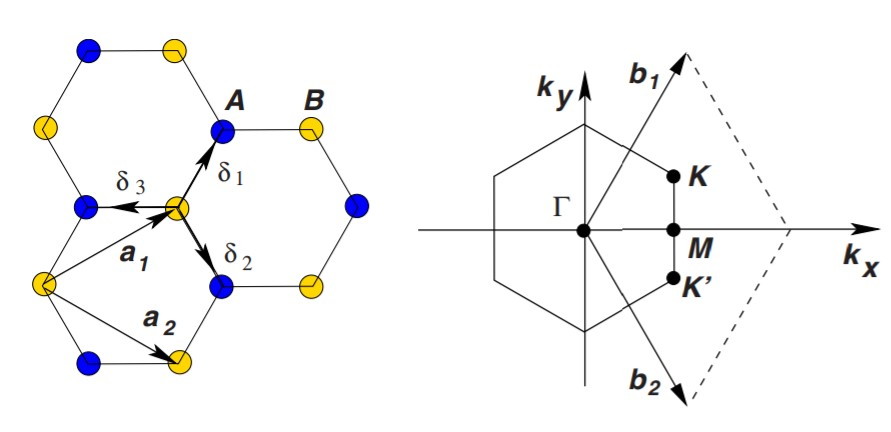
\includegraphics[width=\textwidth]{figures/lattice.jpg}
         \caption{Graphene Lattice and its Brillouin zone. Left: Two interpenetrating triangular lattices forming graphene honeycomb lattice. $a_1$ and $a_2$ are lattice vectors and $\delta_i, i=1,2,3$ are the nearest neighbour vectors. Right: Corresponding Brillouin zone that shows high symmetry points. The Dirac cones are located at $K$ and $K^\prime$ points. Figure adapted from \cite{Geim}}
         \label{fig:lattice}
\end{figure}
The primitive lattice vectors for the lattice are given by (see fig. \ref{fig:lattice}):
\begin{equation}
    a_1 = \frac{a}{2}(3,\sqrt{3}), a_2 = \frac{a}{2}(3,-\sqrt{3})
\end{equation}
The reciprocal lattice vectors are given by (see fig. \ref{fig:lattice}):
\begin{equation}
    b_1 = \frac{2\pi}{3a}(1,\sqrt{3}), b_2 = \frac{2\pi}{3a}(1,-\sqrt{3})
\end{equation}
The wave vectors of the high symmetry points in the first Brillouin zone are given below, where $K$ and $K^{\prime}$ are two nonequivalent corners known as the Dirac points, as shown in fig. \ref{fig:lattice}.
\begin{equation}
    \Gamma = (0,0),K=\frac{2\pi}{3a}(1,\frac{1}{\sqrt{3}}),K^{\prime}=\frac{2\pi}{3a}(1,-\frac{1}{\sqrt{3}}),M=\frac{2\pi}{3a}(1,0)
\end{equation}
The electronic structure of graphene can be derived using the tight binding model, considering nearest and next nearest neighbour hopping. The Hamiltonian becomes:
\begin{equation}
    H= -t\sum_{<i,j>,\sigma}(a_{\sigma,i}^\dagger b_{\sigma,j}+H.c)-t^\prime(a_{\sigma,i}^\dagger a_{\sigma,j}+b_{\sigma,i}^\dagger b_{\sigma,j}+H.c.)
\end{equation}
where $a_{\sigma,i}$, $a_{\sigma,i}^\dagger$ and $b_{\sigma,i}$, $b_{\sigma,i}^\dagger$ are the annihilation and creation operators on site A and B, with spin $\sigma$, respectively. $t$ is the nearest neighbour hopping energy $\approx 2.7eV$ and $t^\prime$ is the next nearest neighbour hopping energy $\approx -0.2 t$. We can diagonalise the Hamiltonian and derive the electronic dispersion to be \cite{Geim}:
\begin{equation}
E_\pm(\mathbf{k})=\pm t \sqrt{f(\mathbf{k})+3}-t^\prime f(\mathbf{k}), f(\mathbf{k})= cos(\frac{\sqrt{3}}{2}k_y a)cos(\frac{3}{2}k_x a )+2cos(\sqrt{3}k_y a)
\end{equation}

\begin{figure}[H]
         \centering
         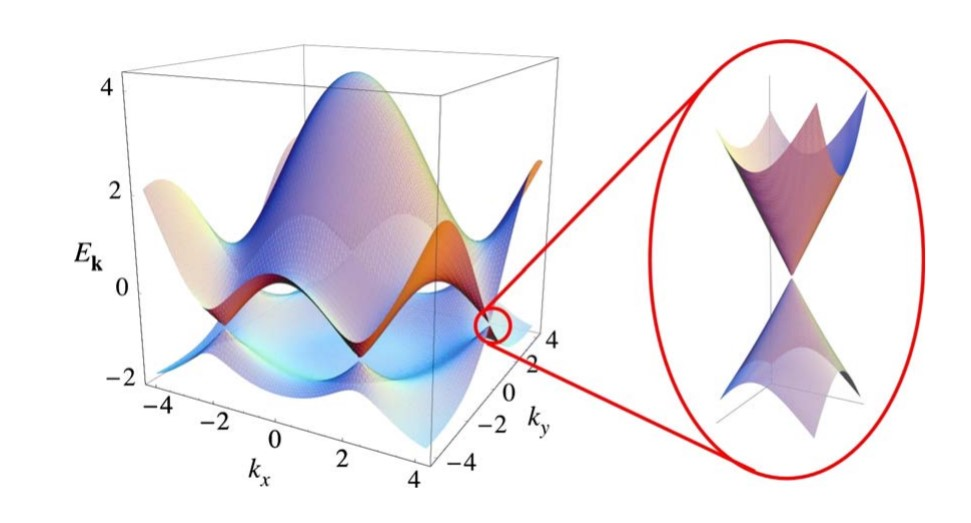
\includegraphics[width=\textwidth]{figures/dispersion.jpg}
         \caption{Electronic dispersion of graphene. Left: Energy spectrum of the honeycomb lattice in units of $t$ for non zero $t$ and $t^\prime$. Here $t=2.7 eV$ and $t^\prime=-0.2t$. Right: Zoom in of the energy bands near one of the Dirac points. Figure adapted from \cite{Geim}}
         \label{fig:dispersion}
\end{figure}
This gives symmetric band structure for holes and electrons around zero energy, if we take $t^\prime$ to be zero. But the electron-hole symmetry is broken and the upper and lower bands become asymmetric for finite next nearest neighbour hopping. In
fig. \ref{fig:dispersion}, the full band structure of graphene is shown. A zoom in of the band structure close to one of the Dirac points is also shown. This dispersion can be
obtained by expanding the full band structure, close to $\mathbf{K}$ or $\mathbf{K^\prime}$ vector, i.e., $\mathbf{k}=\mathbf{K}+\mathbf{q}$ $(|\mathbf{q}|<<\mathbf{K})$:
\begin{equation}
    E_\pm(\mathbf{q})=\pm v_F|\mathbf{q}|+ O[(q/K)^2]
\end{equation}
where $\mathbf{q}$ is the momentum measured relatively to the
Dirac points and $v_F$ is the Fermi velocity, given by $v_F=3ta/ 2$.

The above equation shows that the energy bands linearly cross at the Dirac points and hence the graphene acts as a zero band gap material with a linear dispersion. The approximation is valid for small carrier densities. From equation (2.6), the Hamiltonian near the Dirac points can be written as:
\begin{equation}
    H_{Dirac} =\begin{bmatrix}
0 & q_x-i q_y \\
q_x+i q_y & 0 
\end{bmatrix} = v_F\mathbf{\sigma}.\mathbf{q}
\end{equation}
where $\sigma$ is the corresponding Pauli matrices. This is equivalent to the equation for massless chiral Dirac fermions in 2D where the speed of light has been replaced by $v_F$ and with a pseudospin spinor structure related to the graphene sublattices. Many of the interesting properties of graphene can be explained using this unique and interesting dispersion.

\section{Bilayer Graphene}
  \begin{figure}[H]
         \centering
         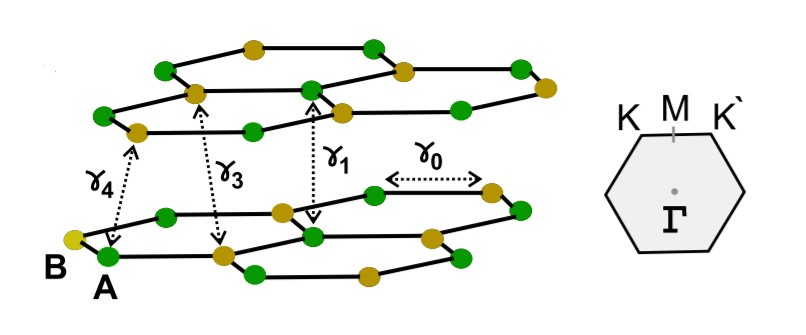
\includegraphics[width=\textwidth]{figures/bilayer_lattice.jpg}
         \caption{Bernal stack bilayer graphene lattice with hopping terms and its Brillouin zone. Left: Two monolayer graphene in AB stacking forming bernal stack bilayer graphene lattice. $\gamma_0$, $\gamma_1$, $\gamma_3$ and $\gamma_4$ are the hopping terms. Right: Corresponding Brillouin zone that shows high symmetry points. Figure adapted from \cite{Geim}}
         \label{fig:bilayer_lattice}
 \end{figure}
Bilayer graphene usually refers to AB stacking or Bernal stacking in which two layers of graphene are stacked on top of each other such that the two layers are shifted by one atomic spacing, as shown in fig. \ref{fig:bilayer_lattice}. The tight binding model gives us the energy dispersion of bilayer graphene. Considering various hopping terms - in-plane nearest neighbour hopping, $\gamma_0\approx2.7 eV$, hopping between atom $A_1$ and atom  $A_2$, $\gamma_1\approx0.4$, hopping between atom $B_1$ and atom $B_2$, $\gamma_1\approx0.3$ and hopping between atom $A_1(A_2)$ and atom $B_2(B_1)$, the tight-binding Hamiltonian becomes:

\begin{align}
\begin{split}
    H & = -\gamma_0\sum_{<i,j>,m,\sigma}(a_{i,m,\sigma}^\dagger b_{j,m,\sigma}+H.c.)-\gamma_1 \sum_{j,\sigma}(a_{j,1,\sigma}^\dagger a_{j,2,\sigma}+H.c.) \\
    & -\gamma_3 \sum_{j,\sigma}(b_{j,1,\sigma}^\dagger b_{j,2,\sigma}+H.c.)-\gamma_4 \sum_{j,\sigma}(a_{j,1,\sigma}^\dagger b_{j,2,\sigma}+a_{j,2,\sigma}^\dagger b_{j,1,\sigma}+H.c.)
\end{split}
\end{align}
where $a_{i,m,\sigma}$($b_{j,m,\sigma}$) annhilates an electron on sublattice $A(B)$ with spin $\sigma$ on plane $m=1,2$. If we apply a perpendicular electric field to the system, an electrochemical potential $\Delta$ is added between the layers. The Hamiltonian in the $k$ space near the $K(K^\prime)$ points, ignoring the weaker hopping terms $\gamma_3$ and $\gamma_4$, can be represented as \cite{Geim}: 
\begin{equation}
    H_{K/K^\prime} = \begin{bmatrix}
    -\frac{\Delta}{2} & v_Fk & 0 & 0 \\
    v_Fk & -\frac{\Delta}{2} & \gamma_1 & 0 \\
    0 & \gamma_1 & \frac{\Delta}{2} & v_Fk \\
    0 & 0 & v_Fk & \frac{\Delta}{2}
\end{bmatrix}
\end{equation}
The resultant electronic dispersion near the Dirac points is given by:
\begin{equation}
    E_\pm^2 = \frac{\Delta^2}{4}+v_F^2k^2+\frac{\gamma_1^2}{2}\pm\sqrt{\Delta^2v_F^2k^2+\gamma_1^2v_F^2k^2+\frac{\gamma_1^4}{4}}
\end{equation}
This equation gives rise to four solutions, hence, four bands near the $K(K^\prime)$ points, as shown in fig. \ref{fig:bilayer_dispersion}. For $\Delta=0$ and  $v_F<<\gamma_1$, the lowest two bands are given by:
\begin{equation}
    E\approx\frac{v_F^2k^2}{\gamma_1}
\end{equation}
We see that even bilayer graphene does not have a band gap when no external displacement field is applied. But unlike monolayer graphene which has a linear dispersion, bilayer graphene has a parabolic dispersion near the Dirac points, with effective mass $m^*=\frac{\gamma_1}{2v_F^2}$.
For $\Delta\neq 0$ and $\Delta<<\gamma_0$, the lowest two bands are given by:
\begin{equation}
    E \approx \frac{\Delta}{2}-\frac{ \Delta v^{2}_{F} k^{2}}{\gamma_1}+\frac{v^{4}_F k^{4}}{ \gamma_1^{2} \Delta}
\end{equation}
In the presence of a displacement field, we see that a band gap opens up, which can be tuned by changing the applied perpendicular electric field.

     \begin{figure}[H]
         \centering
         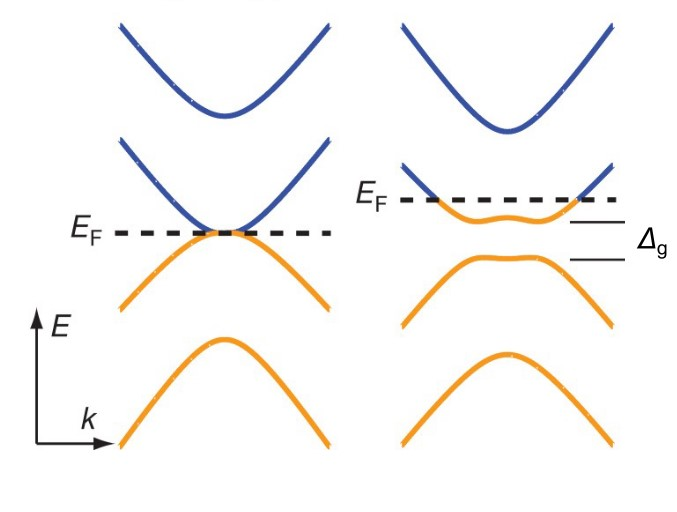
\includegraphics[width=\textwidth]{figures/bilayer_dispersion.jpg}
         \caption{Electronic dispersion of bilayer graphene when $\Delta=0$ (left) and $\Delta\neq0$ (right). A band gap $\Delta_g$ opens up in the presence of an external displacement field. Figure adapted from \cite{Zhang2009}}
         \label{fig:bilayer_dispersion}
     \end{figure}

\section{Twisted Bilayer Graphene}
\subsection{Moire Superlattices}
A geometric interference pattern, known as moire pattern, is formed when two dimensional crystals with a lattice mismatch or a relative twist between them are stacked on top of each other. The wavelength of the moire pattern in case two layers of graphene is given by:
\begin{equation}
    \lambda = \frac{(1+\delta)a}{\sqrt{2(1+\delta)(1-cos\theta)+\delta^2}}
\end{equation}
where $a$ is the lattice constant of graphene, $\theta$ is the twist angle between the two layers and $\delta$ is the lattice mismatch between the two layers. Moire pattern gives rise to effective superlattice potential with a periodicity different from the original lattice. We can see that the moire wavelength becomes much larger than the lattice constant for small twist angles. When $\lambda$ becomes comparable to the Fermi wavelength, the electronic structure is significantly modified. For example, aligned graphene-hBN heterostructures give rise to secondary Dirac points as a result of the moire superlattice potential.
 \begin{figure}[H]
        \centering
         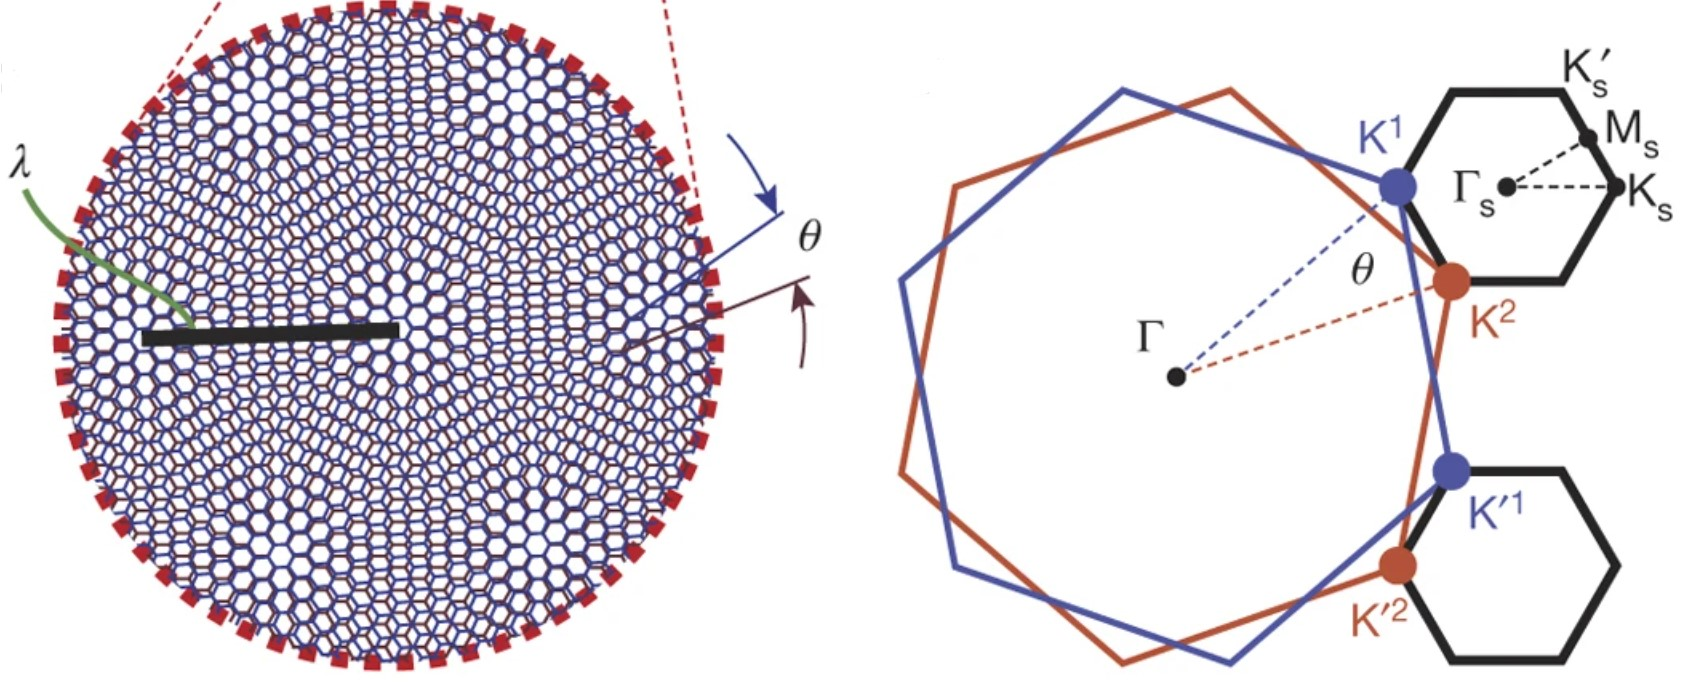
\includegraphics[width=\textwidth]{figures/twblg_lattice.jpg}
         \caption{twBLG moire pattern and its mini Brillouin zone. Left:  The moiré pattern as seen in twBLG. The moiré wavelength is $\lambda=\frac{a}{2sin(\theta/2)}$. Right: The mini Brillouin zone is constructed from the difference between the two $K(K^\prime)$ wavevectors for the two layers. $K_s$,$K_s^\prime$,$M_s$ and $\Gamma_s$ denote points in the mini Brillouin zone. Figure adapted from \cite{Cao2018}}
         \label{fig:twblg_lattice}
\end{figure}

\subsection{Continuum Model}
The geometry of the bilayer system is characterised by a twist angle $\theta$ and a translation vector $\mathbf{d}$. But commensurability is determined only by the twist angle. In a commensurate structure, sliding one layer with respect to another modifies the unit cell but leaves the bilayer crystalline. So, let's consider AB stacking as the aligned configuration. The positions of the carbon atoms in the two layers are then $\mathbf{R}$ and $\mathbf{R^{\prime}} = M(\theta)(\mathbf{R}-\tau)+\mathbf{d}$, where $\tau$ is a vector connecting the two atoms in the unit cell, and $M$ is a two dimensional rotation matrix within the graphene plane.

The bilayer forms a two-dimensional crystal only at a discrete set of commensurate twist angles. Bloch's theorem doesn't apply microscopically at generic twist angles and hence direct electronic structure calculations are not possible. For twist angles larger than a few degrees, except for a small set of angles that give low-order commensurate structure, the two layers are electronically isolated. As the twist angle reduces, interlayer coupling strengthens and quasiparticle velocity at Dirac point decreases. We derive a low-energy effective Hamiltonian valid for any value of $\mathbf{d}$ and for small twist angles, $\theta<10^o$ \cite{Bistritzer12233}.
\begin{figure}[H]
    \centering
     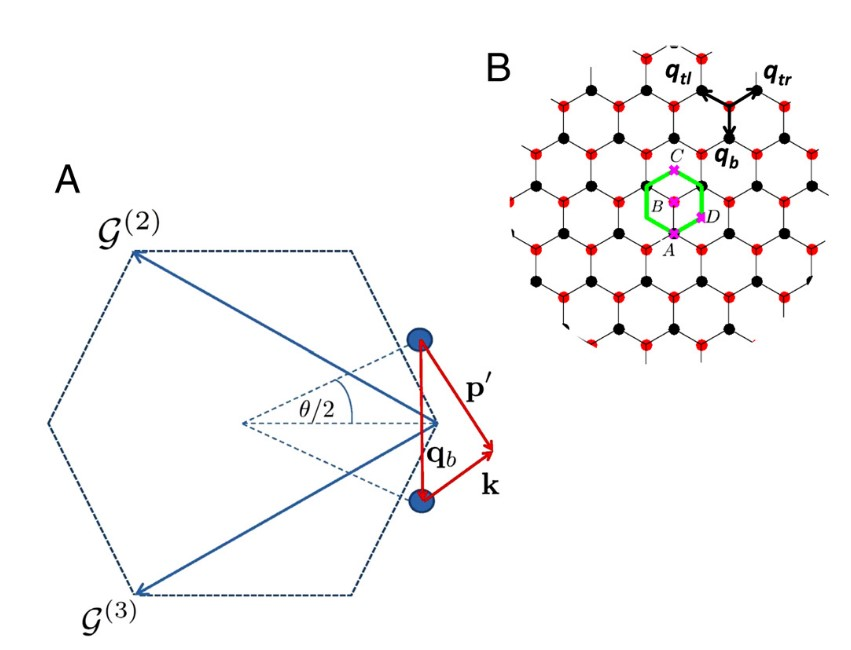
\includegraphics[width=\textwidth]{figures/contmodel.jpg}
     \caption{Cont. Figure adapted from \cite{Bistritzer12233}}
     \label{fig:contmodel}
\end{figure}
The low-energy continuum model Hamiltonian has three terms: two single-layer Dirac-Hamiltonian terms that are associated with the isolated graphene sheets and a tunneling term that accounts for the hopping between the layers. The Dirac-Hamiltonian for a layer rotated by an angle $\theta$ with respect to a fixed coordinate system is given by \cite{Geim}:
\begin{equation}
    h_{\mathbf{k}}(\theta)=-vk \begin{bmatrix}
        0 & e^{i(\theta_{\mathbf{k}}-\theta)}\\
        e^{-i(\theta_{\mathbf{k}}-\theta)} & 0 
    \end{bmatrix}
\end{equation}
where $\mathbf{k}$ is the momentum measured from the Dirac point, $v$ is the Dirac velocity, $\theta_{\mathbf{k}}$ is the momentum orientation relative to the x axis. Choosing the coordinate system as shown in fig. \ref{fig:contmodel}, the decoupled bilayer Hamiltonian is $|1>h(\theta/2)<1|+|2>h(-\theta/2)<2|$, where $<i||i>$ projects onto layer $i$.

Assuming that the interlayer tunneling amplitude between the $\pi$-orbitals is a smooth function of spatial seperation projected onto the graphene planes, we derive a continuum model. The matrix element,
\begin{equation}
    T_{\mathbf{kp^\prime}}^{\alpha\beta}=<\Psi_{\mathbf{k}\alpha}^{(1)}|H_T|\Psi_{\mathbf{p\prime}\beta}^{(2)}>
\end{equation}
of the tunneling Hamiltonian $H_T$, describes a process in which an electron with momentum $\mathbf{p\prime}=M\mathbf{p}$ on sublattice $\beta$ in one layer hops to a momentum $\mathbf{k}$ on sublattice $\alpha$ in the other layer.

In a $pi$-band tight-binding model the projection of the wavefunctions of the two layers onto a given sublattice are:
\begin{equation}
    |\psi_{\mathbf{k} \alpha}^{(1)}>=\frac{1}{\sqrt{N}} \sum_{\mathbf{R}} e^{i \mathbf{k}\left(R+\tau_{\alpha}\right)}|\mathbf{R}+\tau_{\alpha}>
\end{equation}
and
\begin{equation}
    |\psi_{\mathbf{p} \beta}^{(2)}>=\frac{1}{\sqrt{N}} \sum_{\mathbf{R}^{\prime}} e^{i \mathbf{p}\left(R^{\prime}+\tau_{\beta}^{\prime}\right)}|\mathbf{R}^{\prime}+\tau_{\beta}^{\prime}>
\end{equation}
In our case, $tau_{\alpha}=0$, $\tau_{\beta}=\tau$, and $\mathbf{R}$ is summed over the triangular Bravais lattice. Using the above equations and the two-center approximation, we get,
\begin{equation}
    <\mathbf{R}+\tau_{\alpha}|H_T|\mathbf{R}^\prime +\tau_{\beta}^\prime>=t(\mathbf{R}+\tau_{\alpha}-\mathbf{R}^\prime - \tau_{\beta}^\prime)
\end{equation}
for the interlayer hopping amplitude in which $t$ depends on the difference between the positions of the two carbon atoms. We find that
\begin{equation}
T_{\mathbf{k p}^{\prime}}^{\alpha \beta}=\sum_{\mathbf{G}_{1} \mathbf{G}_{2}} \frac{t_{\overline{\mathbf{k}}+\mathbf{G}_{1}}}{\Omega} e^{i\left[\mathbf{G}_{1} \tau_{\alpha}-\mathbf{G}_{2}\left(\tau_{\beta}-\tau\right)-\mathbf{G}_{2}^{\prime} \mathbf{d}\right]} \delta_{\overline{\mathbf{k}}+\mathbf{G}_{1}, \overline{\mathbf{p}}^{\prime}+\mathbf{G}_{2}^{\prime}}
\end{equation}
where, $\Omega$ is the unit cell area, $t_{\mathbf{q}}$ is the Fourier transform of the tunneling amplitude $t(\mathbf{r})$, the vectors $\mathbf{G_1}$ and $\mathbf{G_2}$ are summed over reciprocal lattice vectors, and $\mathbf{G_2}^\prime = M \mathbf{G_2}$. Here, momentum is measured relative to the center of the Brillouin zone and not relative to the Dirac point.

The continuum model for $H_T$ is obtained by measuring wave vectors in both layers relative to their Dirac points and assuming that the deviations are small compared to Brillouin-zone dimensions. Although $t_q$ is not precisely known, it should fall to zero very rapidly with $q$ on the reciprocal lattice vector scale. This is because the graphene layer seperation exceeds the seperation betweeen carbon atoms in a layer by more than twice.

The largest $t_q$ values that enter the tunneling near the Dirac point have $q=k_D$, the Brillouin-zone corner (Dirac) wave vector magnitude, and correspond to the three reciprocal vectors 0, $G^{(2)}$, and $G^{(3)}$ where the latter two vectors connect a Dirac point with its equivalent first Brillouin-zone counterparts (See fig. \ref{fig:contmodel}). When only these terms are retained, we get,
\begin{equation}
T^{\alpha \beta}(\mathbf{r})=w \sum_{j=1}^{3} \exp \left(-i \mathbf{q}_{j} \cdot \mathbf{r}\right) T_{j}^{\alpha \beta}
\end{equation}
where $w=t_{k_D}/\Omega$ is the hopping energy,

\begin{align}
	T_1 = \begin{bmatrix}
		1 & 1 \\
		1 & 1
	\end{bmatrix} &&
	T_2=e^{-i \mathscr{G}^{(2)\prime} \cdot \mathbf{d}} \begin{bmatrix}
		e^{-i \phi} & 1 \\ e^{i \phi} & e^{-i \phi}
	\end{bmatrix} &&
	T_3=e^{-i \mathscr{G}^{(3)\prime} \cdot \mathbf{d}} \begin{bmatrix}
		e^{i \phi} & 1 \\ e^{-i \phi} & e^{i \phi}
	\end{bmatrix}
\end{align}
and $\phi=2/3$. The three $\mathbf{q}_j$’s are Dirac model momentum transfers that correspond to the three interlayer hopping processes. For $\mathbf{d}=0$ and a vanishing twist angle the continuum tunneling matrix is $3w\delta_{\alpha A}\delta_{\beta B}$, independent of position.

\begin{figure}[H]
	\centering
	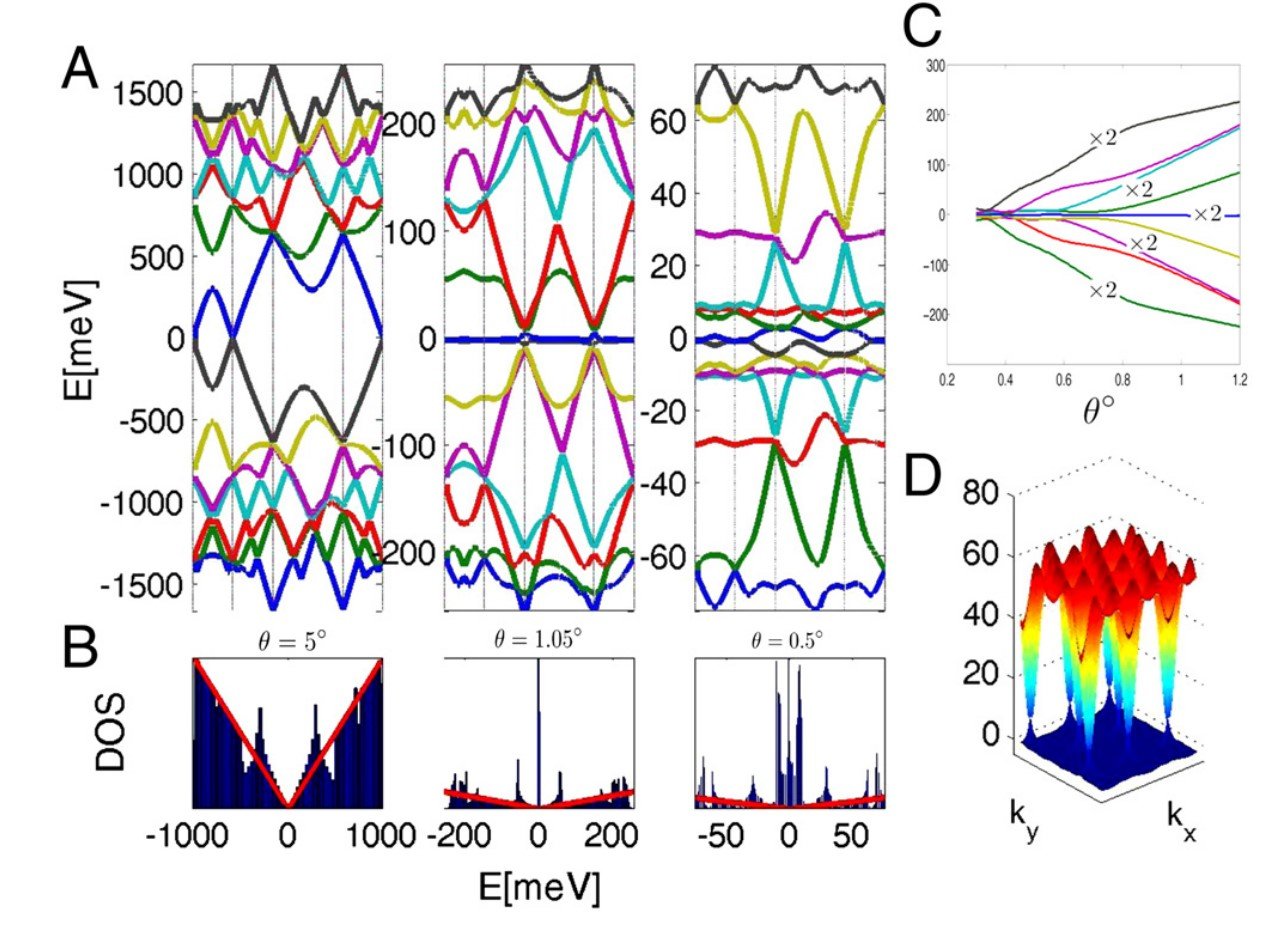
\includegraphics[width=\textwidth]{figures/contmodelband.jpg}
	\caption{Cont. Figure adapted from \cite{Bistritzer12233}}
	\label{fig:contmodelband}
\end{figure}

In the continuum model hopping is local and periodic, allowing Bloch’s theorem to be applied at any rotation angle irrespective of whether or not the bilayer is crystalline. Solving  the moiré bands numerically using the plane wave expansion illustrated in fig. , convergence is attained by truncating momentum space at lattice vectors of the order of $w/\hbar v$. 

Up to a scale factor the moiré bands depend on a single parameter, $\alpha=w/vk_\theta$. Evaluating the moiré bands as a function of their Brillouin-zone momentum $\mathbf{k}$ for different twist angles, we get results as shown in fig. . For large twist angles the low-energy spectrum is virtually identical to that of an isolated graphene sheet, except that the velocity is slightly renormalized. Large interlayer coupling effects appear only near the high energy van Hove singularities discussed by Andrei.

As the twist angle is reduced, the number of bands in a given energy window increases and the band at the Dirac point narrows. As illustrated in fig., we instead find that the Dirac-point velocity vanishes already at $\theta \approx 1.05^o$, and that the vanishing velocity is accompanied by a very flat moiré band which contributes a sharp peak to the Dirac-point density-of-states (DOS). At smaller twists the Dirac-point velocity has a nonmonotonic dependence on twist angle, vanishing repeatedly at the series of magic angles illustrated in fig. .

\begin{figure}[H]
	\centering
	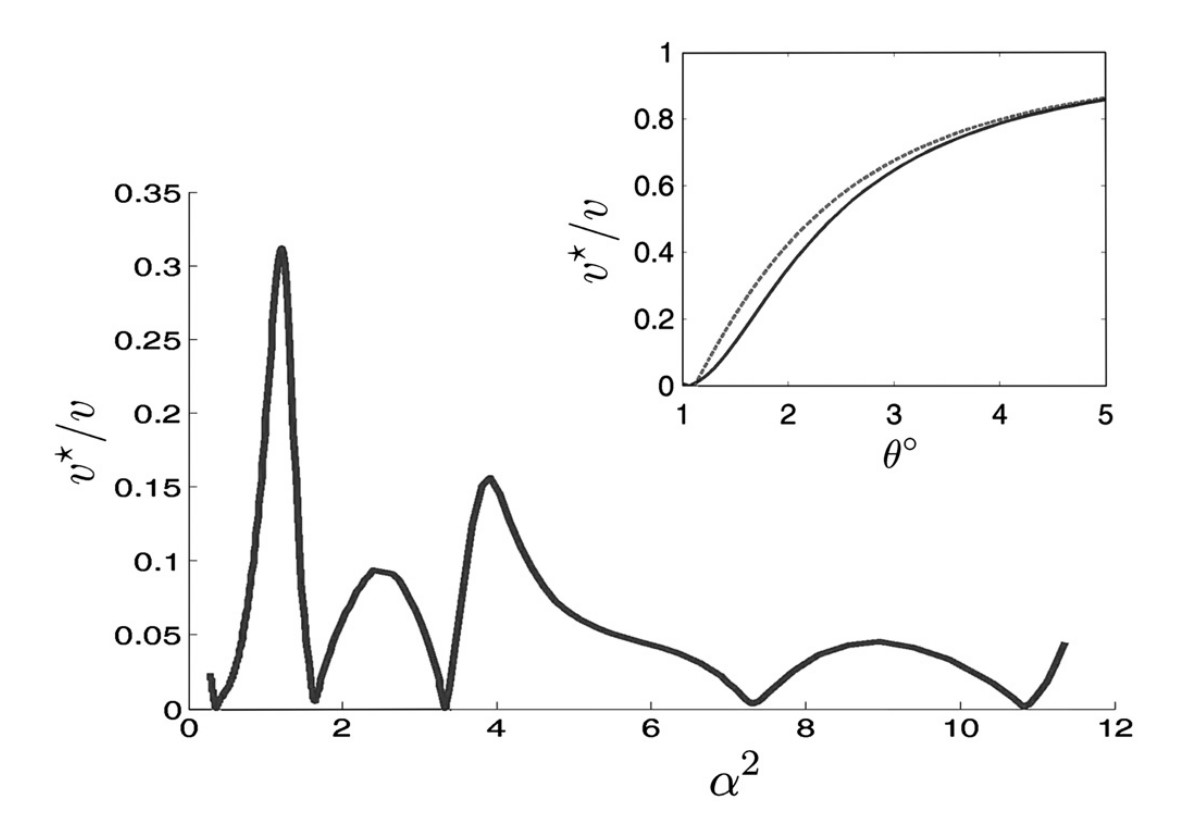
\includegraphics[width=\textwidth]{figures/contmodelvel.jpg}
	\caption{Cont. Figure adapted from \cite{Bistritzer12233}}
	\label{fig:contmodelvel}
\end{figure}

\subsection{Flat bands in twBLG}
Two graphene layers twisted at an angle with respect to each other gives rise to the formation of a mini Brillouin zone. The twist angle $\theta$ displaces the individual monolayer Dirac points by a wave-vector $|k_\theta|=2|K|sin(\theta/2)$, hence forming the mini BZ.

There is hybridisation of the moire bands leading to gap openings at the intersection of the Dirac cones and renormalisation of the Fermi velocity due to the interlayer coupling between the two graaphene layers. A series of magic angles, $\theta=1.05^o, 0.5^o, ...$ have been found at which the Fermi velocity at the Dirac points vanishes that gives rise to flat moire bands with large density of states. The flat bands are formed as a result of competition between the interlayer hybridisation energy and the kinetic energy. When the hybridisation energy, $2w$, becomes comparable to the kinetic energy, $\hbar v_Fk_\theta$, the lower hybridised states are moved to zero energy leading to bands with very narrow band width.
\begin{figure}[H]
     \centering
     \begin{subfigure}[b]{0.8\textwidth}
         \centering
         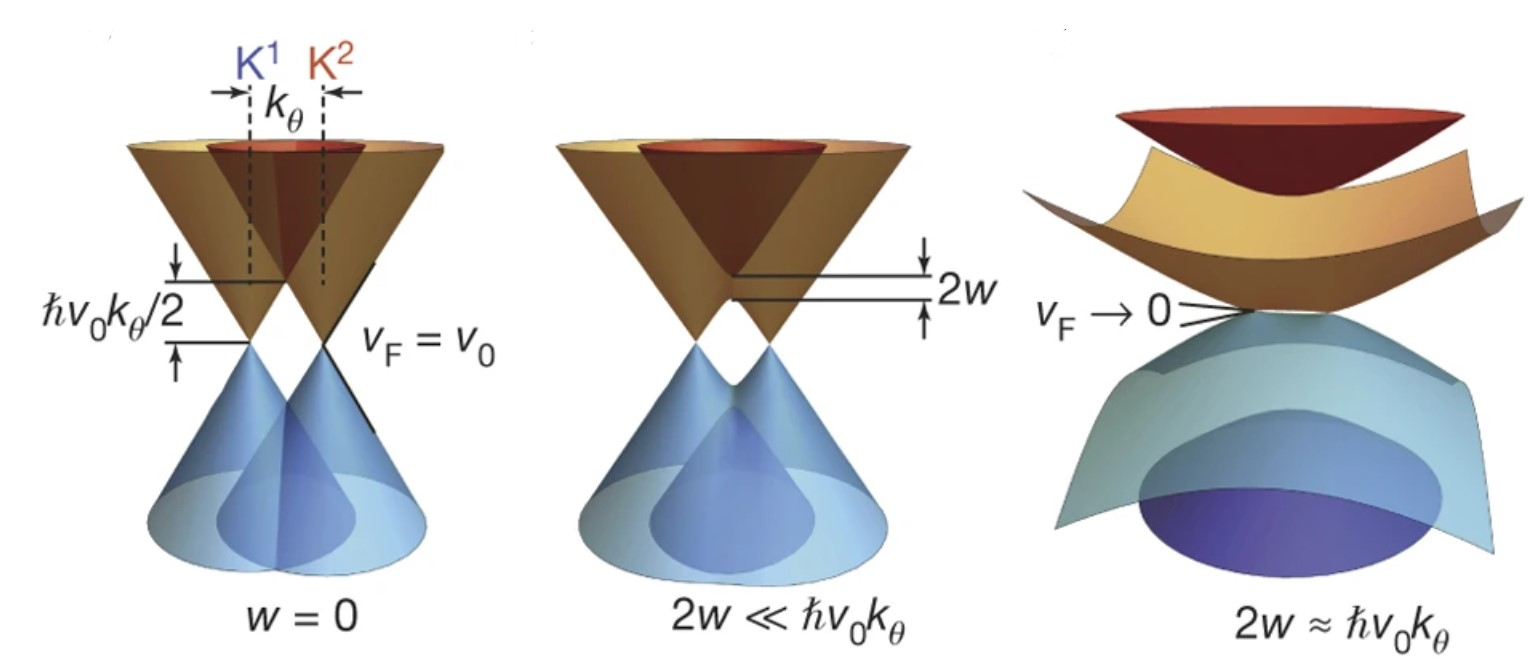
\includegraphics[width=\textwidth]{figures/twblg_hyb.jpg}
         \caption{Illustration of the effect of interlayer hybridization for $w=0$, $2w<<\hbar v_0 k_\theta$ and $2w\approx \hbar v_0 k_\theta$, where $v_0=10^6ms^{-1}$ is the Fermi velocity of graphene. Figure adapted from \cite{Cao2018}}
     \end{subfigure}
     
     \begin{subfigure}[b]{0.8\textwidth}
         \centering
         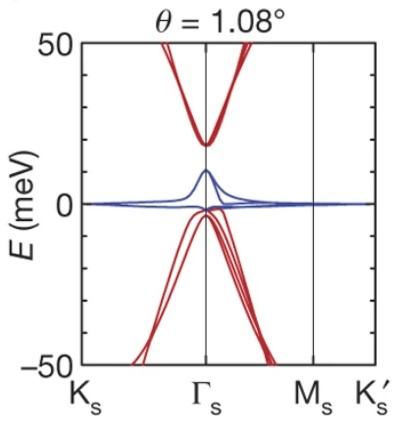
\includegraphics[width=0.5\textwidth]{figures/flatband.jpg}
         \caption{The band energy E of magic-angle ($\theta=1.08^o$) TBG calculated using tight-binding method. The bands shown in blue are the flat bands. Figure adapted from \cite{Cao2018}}
     \end{subfigure}
\caption{Electronic band structure of twBLG}
\end{figure}

\subsection{Experimental Signatures of twBLG}
The single particle picture breaks down, due to the presence of flat bands with large density of states near the charge neutrality point, because the Coulomb interactions exceed the kinetic energy in the system. twBLG enters various strongly correlated and topological states, when the Fermi energy is tuned within the flat bands. It has been experimentally observed to show correlated insulating states, superconductivity, quantum anomalous Hall effect and ferromagnetism.

Each moire superlattice band is four-fold degenerate at low twist angles. The charge density required to fill one superlattice band is given by:
\begin{equation}
    n_s=\frac{4}{A}=\frac{8\theta^2}{\sqrt{3}a^2}
\end{equation}
where $A$ is the area of the moire unit cell. The filling factor, $v=4n/n_s$ gives the number of electrons per moire unit cell. We see from the fig. \ref{fig:twBLG} the presence of resistance peaks at full filling ($v=4$), quarter ($v=1$), half ($v=2$) and three-quarter filling ($v=3$). The insulating states at the full filling are due to the superlattice gap, i.e., it is a band insulator. But the insulating states at quarter, half and three-quarter filling are due to electronic correlations, hence termed correlated insulator. Near the correlated insulating states, the resistance goes to zero, showing the presence of superconducting states. The similarity of these superconducting states to the cuprates suggests a unconventional electronic origin to the superconductivity.

 \begin{figure}[H]
        \centering
         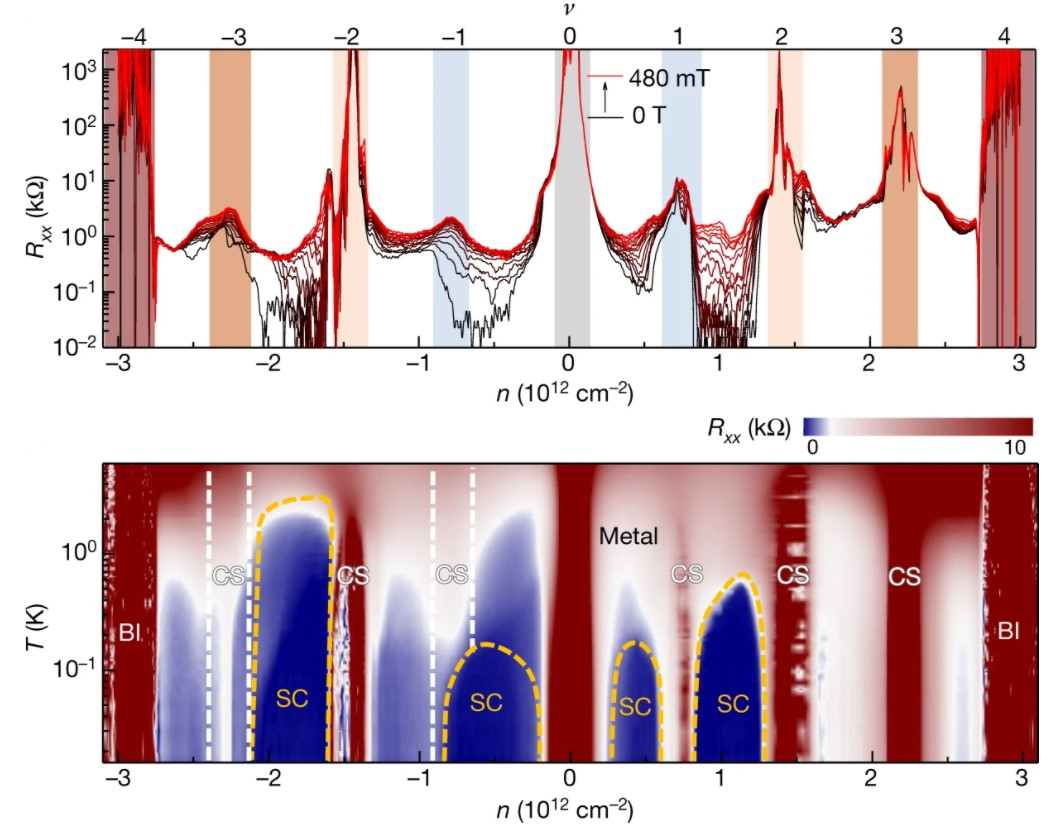
\includegraphics[width=0.8\textwidth]{figures/res_phase.jpg}
         \caption{twBLG transport signatures. Top:  Four-terminal longitudinal resistance plotted against carrier density at different perpendicular magnetic fields from 0 T (black trace) to 480 mT (red trace). Bottom:  Colour plot of longitudinal resistance against carrier density and temperature, showing different phases including metal, band insulator (BI), correlated state (CS) and superconducting state (SC). Figure adapted from \cite{Lu2019}}
         \label{fig:twBLG}
\end{figure}